\documentclass[12pt,titlepage]{scrreprt}
\usepackage[ngerman]{babel}
\usepackage[utf8]{inputenc}
\usepackage{color}
\usepackage{float}
\usepackage[a4paper,lmargin={2.5cm},rmargin={2.5cm},tmargin={2.5cm},bmargin = {2cm}]{geometry}
\usepackage{amssymb}
\usepackage{amsthm}
\usepackage{graphicx}
\usepackage{subfig}
\usepackage{wrapfig}
\usepackage{url}
\usepackage{cite}
\graphicspath{{Images/}}

\begin{document}
% % Activate the following line by filling in the right side. If for example the name of the root file is Main.tex, write
% "...root = Main.tex" if the chapter file is in the same directory, and "...root = ../Main.tex" if the chapter is in a subdirectory.
 
%!TEX root =  TNTinderSee.tex

% mehrere Bilder in einer Bildumgebung mit 
%\subfloat{bild.jpg}


\begin{titlepage}
\thispagestyle{empty}
 \begin{center}
 \begin{figure}[htbp]
    \centering
 %   \subfloat{\includegraphics[width=0.15\textwidth]{Bilder/Titel/bild-firma.JPG}}\quad
   %  \subfloat{\includegraphics[width=0.25\textwidth]{Bilder/Titel/bild-uni 
%oder fh.JPG}}
\end{figure}
\vspace*{1cm}
 \Large{Schiller-Gymnasium Offenburg }

  \vspace*{1.5cm}
 {\huge Thema}
 \vspace*{1cm} \\
 {\Large Abschlussbereicht\\von\\Eitel, Martin \\ \texttt{marjelly1@gmail.com}\\Komyakov, Alexander \\\texttt{alexander.komyakov@lynxisgod.eu} \\ Rehwinkel, Antonio \\ \texttt{antonio.rehwinkel@schiller-og.de} \\ Sauerbrey, Luisa \\ \texttt{luisa.sauerbrey@schiller-og.de}
 \vspace{0.5cm}
 {\Large \bfseries \\}
 \vspace{0.5cm}
 {\Large geboren am dein Geburtstag}
 \vfill
  \vspace*{1.5cm}
\begin{table}[h]
	\centering
	\begin{tabular}{|l| l|}\hline
		Aufgabensteller & Prof. \\ \hline
		Durchgeführt bei: & Firmenname\\ \hline
		Betreuer: & Betreuer Firma\\ Marek Czernohous \\ \hline
		Wissenschaftspate & \\ Prof. Dr. Jens Greinert\\ \hline
		Arbeit vorgelegt am: & Datum\\ \hline
	\end{tabular}
\end{table}
}
\end{center}
\end{titlepage}


\begin{titlepage}

	

\title{Die Auswirkung von Munitionshalden auf die Wasserqualität der Ostsee zwischen Vilm und Lauterbach}
\subtitle{Ausfahrt vom 18.07. - 21.07.2021}
\titlehead{\centering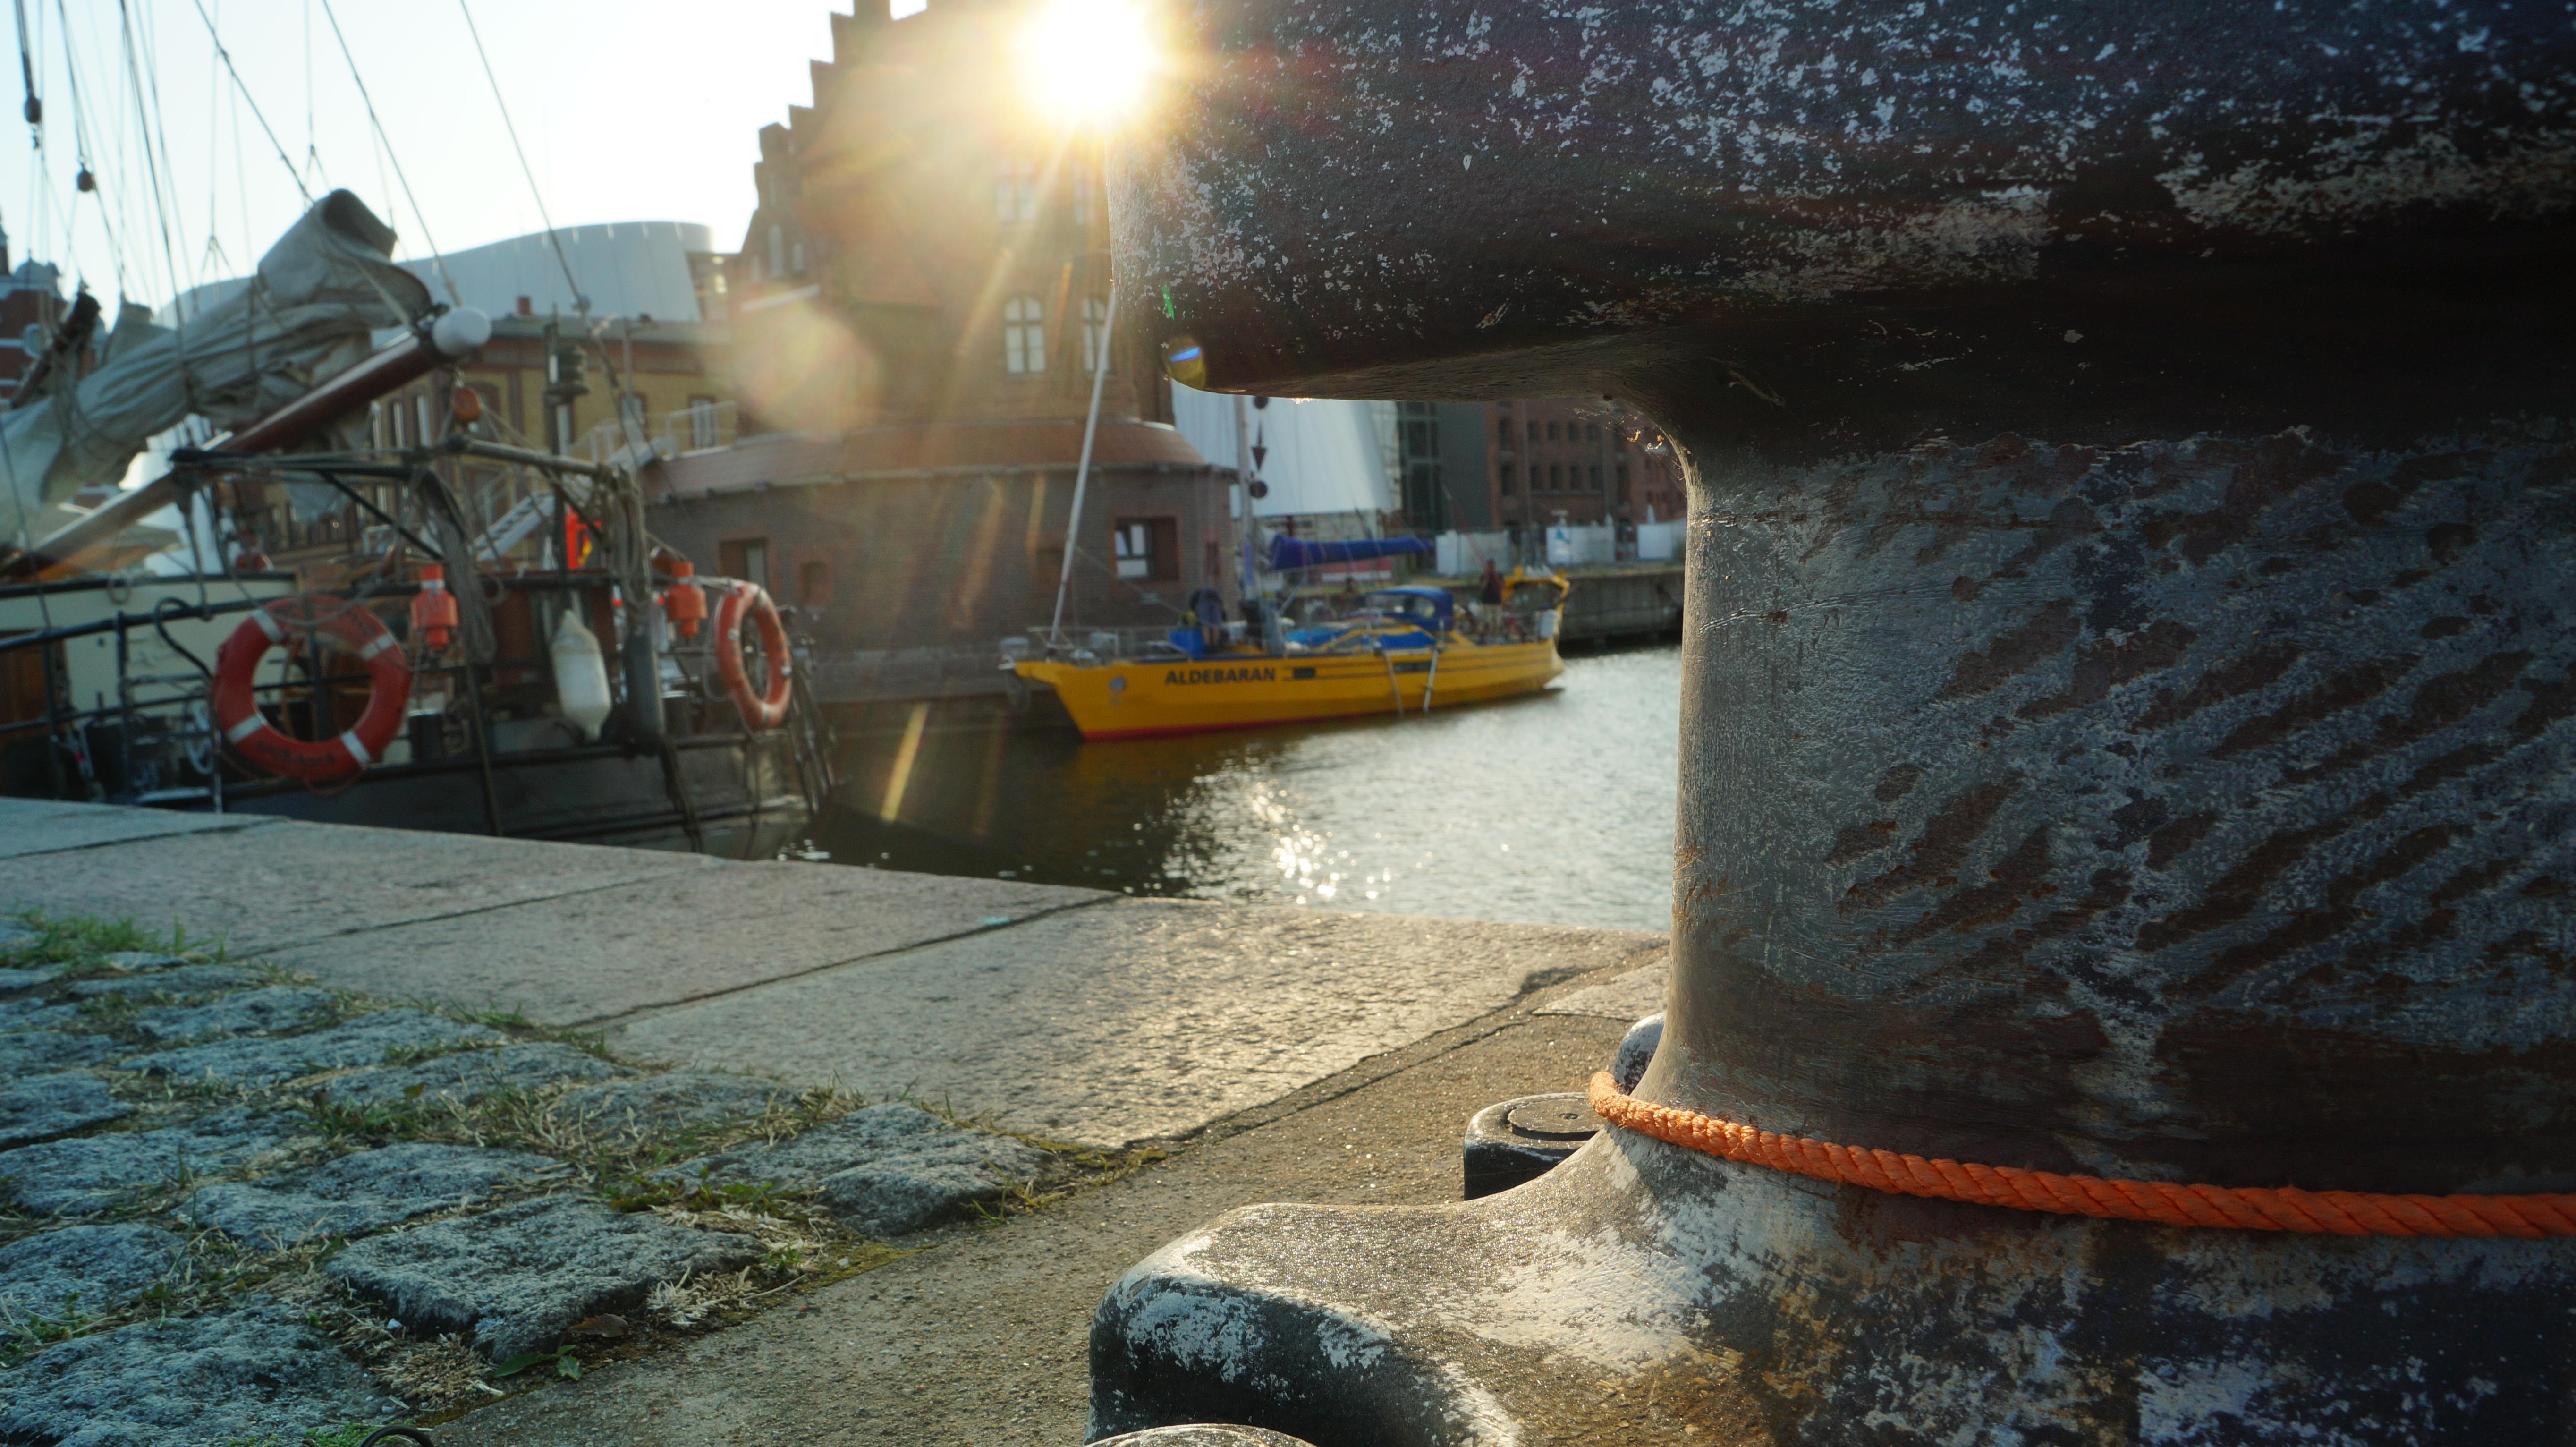
\includegraphics[width=15cm]{Bilder/DSC05220}}


\author{Eitel, Martin; Komyakov, Alexander; \\ Rehwinkel, Antonio; Sauerbrey, Luisa\\ \and Schiller-Gymnasium Offenburg}

\publishers{Wissenschaftspate: Prof Dr. Jens Greinert \texttt{jgreinert@geomar.de} \\
\vspace*{2ex} Betreuer: Marek Czernohous \texttt{m.czernohous@schiller-offenburg.de}}
%- \\ Schiller-Gymnasium Offenburg}

\maketitle

\end{titlepage}
\addchap{Kurzfassung}
Unser Wettbewerbsbeitrag umfasst

\tableofcontents
<<<<<<< HEAD

\chapter{Vorwort}
\section{Vorbedingungen}
\section{Forschungsgegenstand}
\section{Erwartungen}
\chapter{Hauptteil}
\section{Kartierung}
    \subsection*{QGIS}
    Alle Kartierungsvorgänge wurden mit der Free Open Source Software \emph{QGIS}\cite{qgis} durchgeführt.
    \begin{figure}[h]
        \centering
        \includegraphics[width=7cm]{QGIS/about-screenshot.png}
        \caption{QGIS Benutzeroberfläche}
        \label{fig:qgis_scr0}
    \end{figure}
\section{Wasserproben}
\section{Sedimentproben}
\section{Multiparametermessungen}
\section{ROV-Kartierungen}
\section{Fazit}

\begin{thebibliography}{9}
\bibitem{qgis}
QGIS 3.16 LTS
\textit{https://qgis.org/}
\end{thebibliography}

=======
>>>>>>> d20cff3b5620de7e54934cfc8cfe0d4dce294458
% Activate the following line by filling in the right side. If for example the name of the root file is Main.tex, write
% "...root = Main.tex" if the chapter file is in the same directory, and "...root = ../Main.tex" if the chapter is in a subdirectory.
 
%!TEX root =  TNTinderSee.tex

\chapter[Einleitung]{Einleitung}

Im Meer lagernde Munition stellt eine Gefahr dar. Nicht unbedingt durch unmittelbare Detonotationsgefahr, 
sondern durch die langsame Zersetzung, die die enthaltenen Sprengstoffe nach und nach 
freilegt\cite{zeitbomben}. Die Entstehung sprengstofftypischer Abbauprodukte, sowie das direkte Austreten 
giftiger Stoffe, stellen Gesundheitsgefährung exponierter Meerestiere, aber auch Menschen dar, denn die
Abbauprodukte gelten als krebserregend und das potentiell austretende Phosphor lagert sich an den Stränden 
ab und ist von Bernstein kaum zu unterscheiden. Als wir den Meereswettbewerb mit der Aldebaran fanden, 
fühlten wir uns gezwungen nachzuforschen wie groß die Gefahr schon heutzutage ist.\\

Wir wollten in einem potentiellem Munitionsabwurfsgebiet messen, wie groß die Anteile der Schadstoffe sind und 
ob noch etwas von den Granaten und Bomben zu sehen ist. Dazu entschieden wir uns für ein Gebiet kurz Vilm,
da hier angeblich zwei Schuten nach dem Zweiten Weltkrieg mit Munition beladen explodiert sein sollen.\\

Das Naturschutzgebiet Vilm liegt in etwa 100 Meter Entfernung zu der Explosionsstelle und auch weiter 
entfernte Orte können durch Ablagerungen und Schadstoffe in Fisch-Fängen betroffen sein.\\

In Zusammenarbeit mit der Aldebaran und dem Geomar wollten wir die Wracks kartieren und die Schadstoffwerte in
der direkten Umgebung messen. Besonders interessant wäre die beförderte Munition gewesen. Die Frage der
Ortung und Untersuchung der möglichen Funde konnten wir zusammen mit dem Geomar lösen. Mithilfe eines 
"Multibeams" sollten wir interessante Orte ohne Tauchgang finden können um später mit dem Schuleigenen 
ROV die Orte genauer unter die Lupe nehmen zu können. Auch Sedimentproben dirket neben den Fundstätten 
konnten wir mithilfe eines eignene Aufsatzes realisieren.

Wir befürchteten hohe Werte für Phosphor und sprengstofftypische Verbindungen wie Trinitrotoluol (TNT) 
zu messen und unter Umständen sogar Granaten oder Bomben zu finden. Falls dies passieren sollte, würde 
sich für uns die Frage stellen, wie sich diese Munition auf die Öknomie ausgewirkt hat. 

Themenfindung, Relevanz, entscheidende Fragen, Lösungsansätze, Forschungsstand mit Quellen, Erwartungen, konkrete Fragen.

% Activate the following line by filling in the right side. If for example the name of the root file is Main.tex, write
% "...root = Main.tex" if the chapter file is in the same directory, and "...root = ../Main.tex" if the chapter is in a subdirectory.
 
%!TEX root =  TMTinderSee.tex

\chapter[Hauptteil]{Hauptteil}

\section{Kartierung}
    \subsection*{QGIS}
    Die Kartierungsvorgänge wurden alle mit der Free Open Source Software \emph{QGIS}\cite{qgis} durchgeführt.
    
\section{Wasserproben}
\section{Sedimentproben}
\section{Multiparametermessungen}
\section{ROV-Kartierungen}

%!TEX root = TNTinderSee.tex 

\chapter[Fazit]{Fazit}

Obwohl unser Untersuchungsgebiet in einem auf Seekarten als \emph{munitionsbelastetem Gebiet} lag, haben wir trotz aufwändiger Kartierung keine Munition gefunden. Zusätzlich haben uns unsere Wasserproben keinerlei Hinweise sprengstofftypischen Verbindungen, wie man sie in der Nähe von vor-sich-hin rostender Munition erwartet, gezeigt. Betrachtet man die Ergebnisse, wäre die gute Nachricht, dass nicht nur das Gewässer südöstlich von Rügen diesbezüglich unbelastet ist und auch von eventuell nicht aufgespürte Munitionsreste keine Gefahr für das Untersuchungsgebiet zu sein scheint. \\
Andere Untersuchungen kommen allerdings zu anderen Schlüssen, so gilt die Munitionshalde \emph{Kohlberger Heide} in der Kieler Bucht als hochbelastet\cite{kohl} \\
Letztendlich sind unsere Ergebnisse deshalb mit Vorsicht zu interpretieren. \\
Eine plausible Erklärung für unsere Ergebnisse wäre, dass die Reste des o.g. Schutenunglücks zu DDR-Zeiten wieder geborgen wurden und wir deshalb am Ort des Unglücks keine Überreste der Schuten oder der Munition mehr gefunden haben.
Zusätzlich könnte die durch das Flachwasser großzügig vorhandene Biomasse eventuelle Restbelastungen aufgenommen haben. Diese spielt in der Ionenchromatografie wegen der notwendigen Filtrierung der Proben nämlich keine Rolle. \\
Um das zu prüfen, müsste die Biomasse gezielt untersucht werden.\\
Vielleicht waren wir aber auch einfach zu weit weg von der nächsten Munitionshalde.\\
\begin{figure}[htb!]
\includegraphics[height=\textheight,%
                   width=\textwidth,%
                   keepaspectratio]{Bilder/karte_muni.PDF}
\caption{Karte der Munitionslagerstätten in Nord- und Ostsee\cite{shmuni}.}
\end{figure}

Trotz unserer Untersuchungsergebnisse bleibt die Gefahr durch Altmunition in der Ostsee weiter bestehen (siehe Abb 4.1.) und es muss dringend ein Konzept zur Bergung und Entsorgung der Munition her, um das Ökosystem Ostsee zu schützen.\\

Diese Forschungsreise war für uns alle eine wunderbare und sicherlich prägende Erfahrung, dafür möchten wir uns bei allen Beteiligten herzlich bedanken.\\

Und falls bei der nächsten Forschungsfrage ein kleiner Tauchroboter inklusive Minicrew benötigt werden sollte: Wir denken, die See schuldet uns noch was. :-)





% Activate the following line by filling in the right side. If for example the name of the root file is Main.tex, write
% "...root = Main.tex" if the chapter file is in the same directory, and "...root = ../Main.tex" if the chapter is in a subdirectory.
 
%!TEX root =  TNTinderSee.tex

\chapter[Danksagungen]{Danksagungen}
Wir danken Prof Dr. Jens Greinert vom GEOMAR Kiel und Leiter der Arbeitsgruppe DeepSea-Monitoring. Er ist der beste Wissenschaftspate, den wir uns hätten wünschen können.\\
Frank Schweikert und Dr. Hannes Imhof, für die tollen Tage und all die Hilfe an Board der Aldebaran. \\

Mareike Kampmeier für die geduldige Einführung am Multibeam und die vielen Erklärungen zum Thema Sprengstoffe im Wasser. \\

Dr. Inken Suck, die bestimmt coolste ROV-Pilotin



Frank Schweikert und Dr. Hannes Imhof von der deutschen Meeresstiftung, für die tollen Tage und all die Hilfe an Board der Aldebaran. \\


Mareike Kampmeier vom GEOMAR Kiel für die geduldige Einführung am Multibeam und die vielen Erklärungen zum Thema Sprengstoffe im Wasser. \\


Dr. rer. nat. Inken Suck vom GEOMAR Kiel, der bestimmt coolsten ROV-Piloten dafür, dass sie uns gezeigt hat, wie man Unterwasserfahrzeuge richtig navigiert. \\


Maria Martinez Cabanas vom GEOMAR Kiel dafür, dass sie uns und unsere Proben in Ihre Labore mitgenommen hat, und geduldig stundenlang alle Fragen beantwortet hat.\\


Dr. Kevin Köser vom GEOMAR Kiel für den inspirierenden Vortrag über Photogrammetrie \\


Yifan Song vom GEOMAR Kiel dafür, dass er uns ganz praktisch beigebracht hat, wie man Videomaterial georeferenziert.\\


Marek Czernohous für die insgesamt über 24 Stunden Fahrzeit, die Mate, Franzbrötchen und enorme Hilfe beim \LaTeX -Satz.\\



\bibliography{bibliography}
\bibliographystyle{plain}
<<<<<<< HEAD
=======
\include{Anhang}
>>>>>>> d20cff3b5620de7e54934cfc8cfe0d4dce294458
\end{document}
